\documentclass[8pt]{beamer}


\usepackage{beamerthemeMunichHH}
\usepackage{amsmath,amssymb,amsthm}
\usepackage{verbatim,fancyvrb}

\usepackage{graphicx}
\usepackage{wrapfig}
\usepackage{caption}
\usepackage{subcaption}
\usepackage[utf8]{inputenc}
\usepackage[german]{babel}
\usepackage[babel, german=quotes]{csquotes}
\usepackage{hyperref}
\usepackage[style=alphabetic]{biblatex}

\addbibresource{bibliography.bib}

% ------------------------------------------------------------------------
% font management
% ------------------------------------------------------------------------

\usepackage{euler}
\renewcommand{\familydefault}{\sfdefault}
\renewcommand{\rmdefault}{\familydefault}

\usepackage{mathrsfs} % for mathscr font

% ------------------------------------------------------------------------
% References Logistics
% ------------------------------------------------------------------------

\usepackage{lmodern}    
\usepackage[labelformat=empty,font=scriptsize,skip=0pt,justification=justified,singlelinecheck=false]{caption}

%remove the icon
\setbeamertemplate{bibliography item}{}

%remove line breaks
\setbeamertemplate{bibliography entry title}{}
\setbeamertemplate{bibliography entry location}{}
\setbeamertemplate{bibliography entry note}{}

%\usepackage[backend=bibtex,style=alphabetic,firstinits=true,sorting=none]{biblatex}

% google(beamer printbibliography icon does not appear)
% https://tex.stackexchange.com/questions/124256/how-do-i-get-numbered-entries-in-a-beamer-bibliography
\setbeamertemplate{bibliography item}{\insertbiblabel}

\bibliography{mainRefs}

\makeatletter
\def\blx@maxline{77}
\makeatother

% ------------------------------------------------------------------------
\title{Support vector machines with kernel methods}
\author{Author \\ TU-Hamburg }
\date{WS 2017-2018} 
% ------------------------------------------------------------------------
 
\setbeamercolor{black30}{fg=black!30}

%--------------------------------------------------------------------------
% macros
% ------------------------------------------------------------------------
\def\cA{{\mathcal A}}
\def\cB{{\mathcal B}}
\def\cE{{\mathcal E}}
\def\cG{{\mathcal G}}
\def\cC{{\mathcal C}}
\def\cM{{\mathcal M}}
\def\cN{{\mathcal N}}
\def\cH{{\mathcal H}}
\def\cU{{\mathcal U}}
\def\cX{{\mathcal X}}
\def\cY{{\mathcal Y}}
\def\cK{{\mathcal K}}
\def\sD{{\mathsf D}}
\def\fJ{{\mathfrak J}}
\def\bU{{\mathbb U}}
\def\bV{{\mathbb V}}
\def\bR{{\mathbb R}}
\def\bT{{\mathbb T}}
\def\scA{{\mathscr A}}
\def\scB{{\mathscr B}}
\def\scC{{\mathscr C}}
\def\scE{{\mathscr E}}
\def\scH{{\mathscr H}}
\def\scX{{\mathscr X}}

% ===================================

\newcommand{\pd}[2]{\frac{\partial#1}{\partial#2}}      %% partial deriv
\newcommand{\pdd}[2]{\frac{\partial^2#1}{\partial#2^2}} %% partial deriv

% ===================================

\def\<#1,#2>{\langle#1,#2\rangle} %% inner product (Dirac not'n)

\newtheorem{thm}{Theorem}[section]
\newtheorem{prop}{Proposition}[section]
\newtheorem{defi}{Definition}[section]
\newtheorem{lemm}{Lemma}[section]
\newtheorem{exmp}{Example}[section]
\newtheorem{conj}{Conjecture}[section]
\newtheorem{seti}{Setting}[section]
\newtheorem{obje}{Objectives}[section]
\newtheorem{frmk}{}[section]


%--------------------------------------------------------------------------
% Beamer logistics 
% ------------------------------------------------------------------------

\setbeamertemplate{navigation symbols}{}
\setbeamertemplate{footline}[page number]{}
\setbeamercovered{transparent}
% the following is automatically updated after two compilations
% \renewcommand{\inserttotalframenumber}{12} 

% =============================================================
% prepare the footnote that will appear in the whole document 
\setbeamerfont{pa}{size=\footnotesize}
\setbeamerfont{pb}{size=\tiny}
\setbeamercolor{bblack40}{bg=black!40}
\setbeamercolor{black40}{fg=black!50}


\setbeamertemplate{footline}
{
\hskip7mm \begin{beamercolorbox}[wd=120mm]{white}
{\usebeamerfont{pb}\usebeamercolor[fg]{black}{
\hskip 110mm  \insertpagenumber\,/\,\inserttotalframenumber}}
\begin{beamercolorbox}[sep=1.5pt,wd=115mm]{white}    \end{beamercolorbox}\par
\end{beamercolorbox}
}

% =============================================================
% prepare logos for initial page 
\pgfdeclareimage[height=1.0cm]{uniHHLogo}{tuhhLogo}
\pgfdeclareimage[height=1.0cm]{depmatLogo}{Mathe-Logo}
\usepackage[absolute,overlay]{textpos}
\setlength{\TPHorizModule}{1mm}
\setlength{\TPVertModule}{1mm}

\newcommand{\MyLogoA}{%
\begin{textblock}{14}(2.0,0.9)
  \pgfuseimage{uniHHLogo}
\end{textblock}
}

\newcommand{\MyLogoB}{%
\begin{textblock}{14}(90.0,0.9)
  \pgfuseimage{depmatLogo}
\end{textblock}
}



\begin{document}

  \frame{\titlepage\MyLogoA\MyLogoB}

  %%%%%%%%%%%%%%%%%%%%%%%%%%%%%%%%%%%%%%%%%%%%%%%%%%%%%%%%%%%%%%%%%%%%%%%%%%%%%%%%
% Folie 1: Motivation
%%%%%%%%%%%%%%%%%%%%%%%%%%%%%%%%%%%%%%%%%%%%%%%%%%%%%%%%%%%%%%%%%%%%%%%%%%%%%%%%
\begin{frame}
    \frametitle{Motivation}

    \begin{figure}[h]
        \centering{
            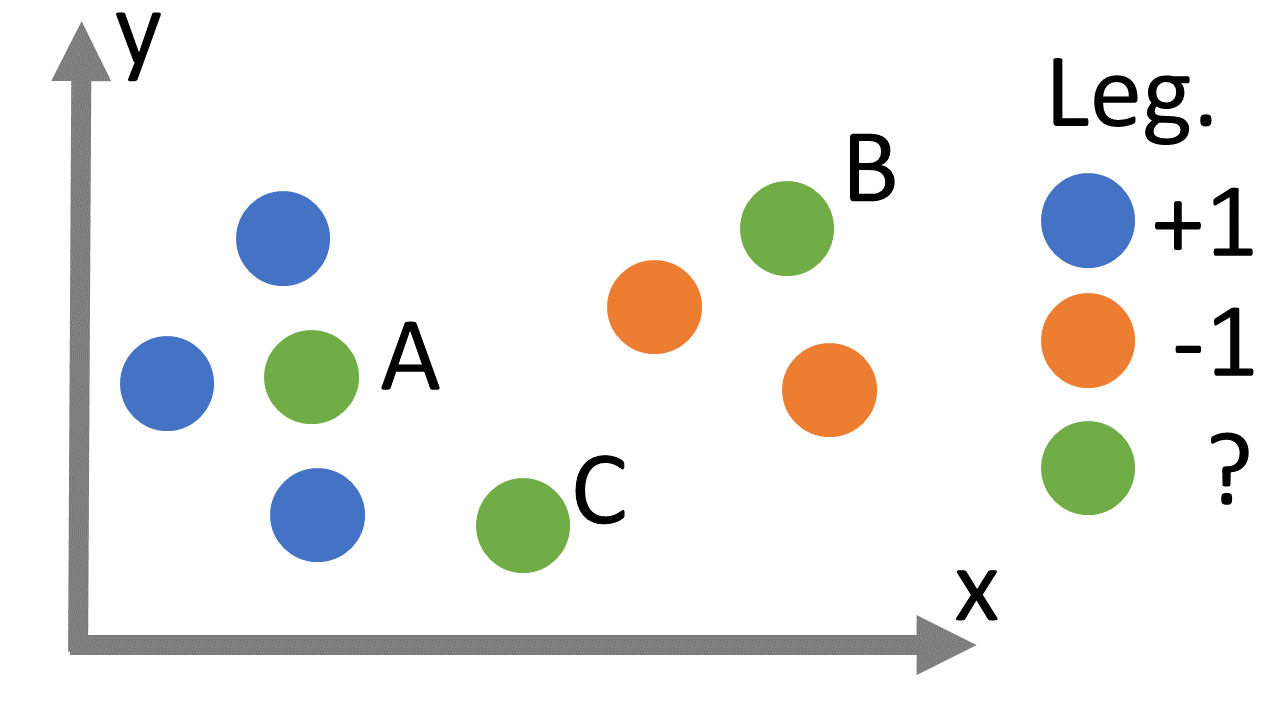
\includegraphics[width=0.5\linewidth]{PowerPoint/Folie1.png}
            % \caption{Beispiel eines Training-Sets mit zu klassifizierenden Punkten}
            \label{motivation:fig_1}
        }
    \end{figure}

    \vspace{3mm}

    \begin{itemize}
        \item Klassifizierung von Objekten
        \item Schnell und effizient
        \item Möglichst genau
    \end{itemize}
\end{frame}

%%%%%%%%%%%%%%%%%%%%%%%%%%%%%%%%%%%%%%%%%%%%%%%%%%%%%%%%%%%%%%%%%%%%%%%%%%%%%%%%
%Folie 2: Themenvorstellung
%%%%%%%%%%%%%%%%%%%%%%%%%%%%%%%%%%%%%%%%%%%%%%%%%%%%%%%%%%%%%%%%%%%%%%%%%%%%%%%%
\begin{frame}
    \frametitle{Themenvorstellung}

    \begin{figure}[h]
        \centering{
            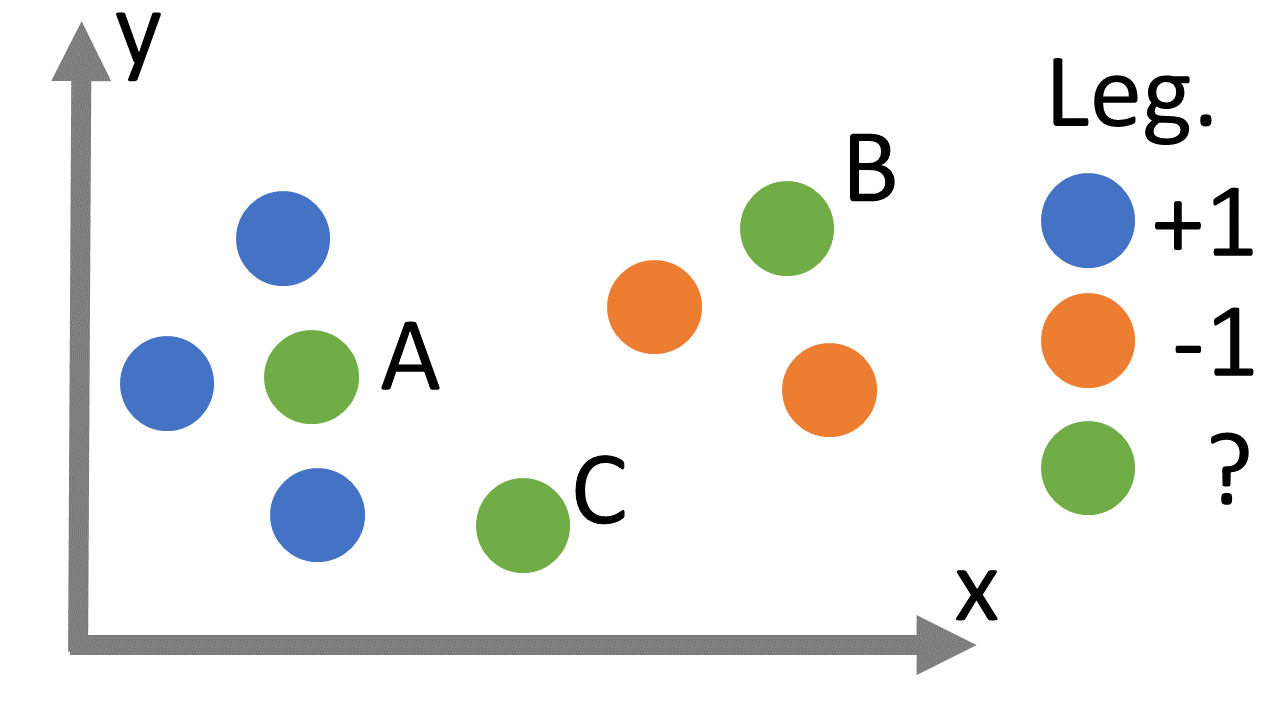
\includegraphics[width=0.5\linewidth]{PowerPoint/Folie1.png}
            % \caption{Beispiel eines Training-Sets mit zu klassifizierenden Punkten}
            \label{themenvorstellung:fig_1}
        }
    \end{figure}

    \vspace{3mm}

    \begin{itemize}
        \item Support Vector Machines (deutsch: Stützvektor Maschine)
        \item Binärer Klassifierierer
    \end{itemize}
\end{frame}

%%%%%%%%%%%%%%%%%%%%%%%%%%%%%%%%%%%%%%%%%%%%%%%%%%%%%%%%%%%%%%%%%%%%%%%%%%%%%%%%
%Folie 3: Lineare Klassifizierung
%%%%%%%%%%%%%%%%%%%%%%%%%%%%%%%%%%%%%%%%%%%%%%%%%%%%%%%%%%%%%%%%%%%%%%%%%%%%%%%%
\begin{frame}
    \frametitle{Lineare Klassifizierung}

    \only<1>{
        \begin{figure}[h]
            \centering{
                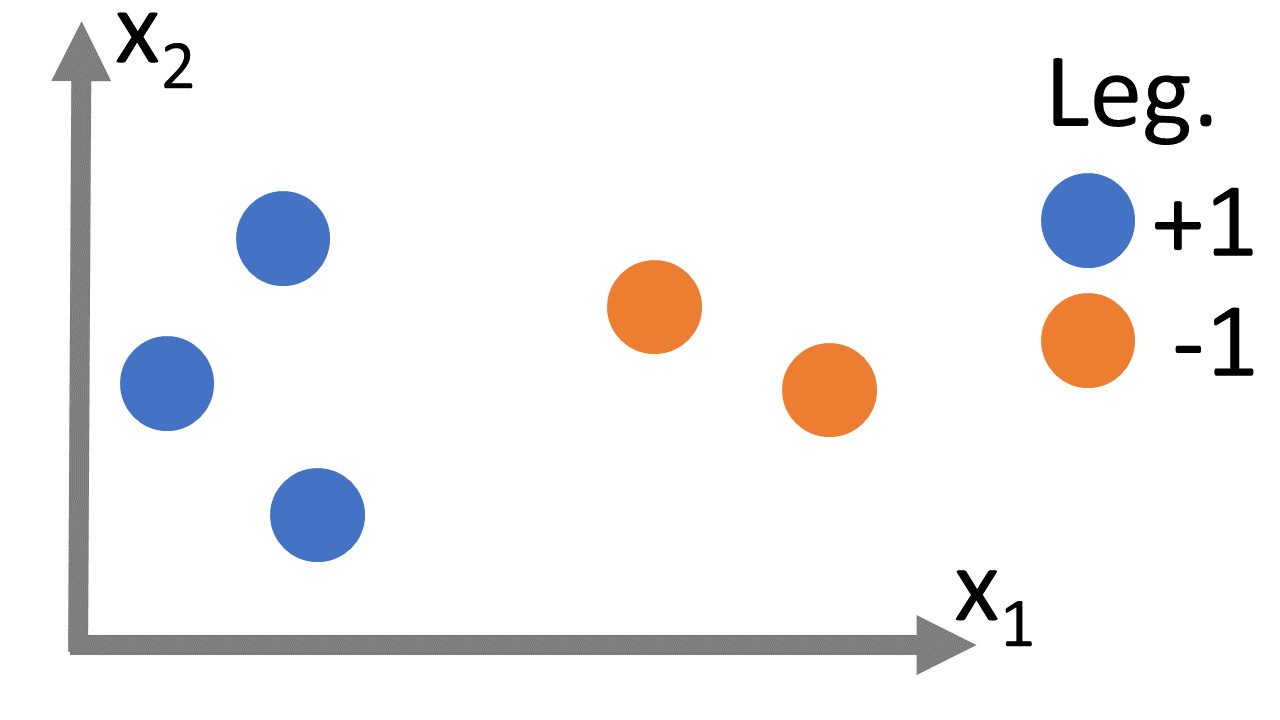
\includegraphics[width=0.5\textwidth]{PowerPoint/Folie2.png}
                % \caption{Beispiel eines Training-Sets}
                \label{lin_klassif:fig_1}
            }
        \end{figure}
    }\only<2>{
        \begin{figure}[h]
            \centering{
                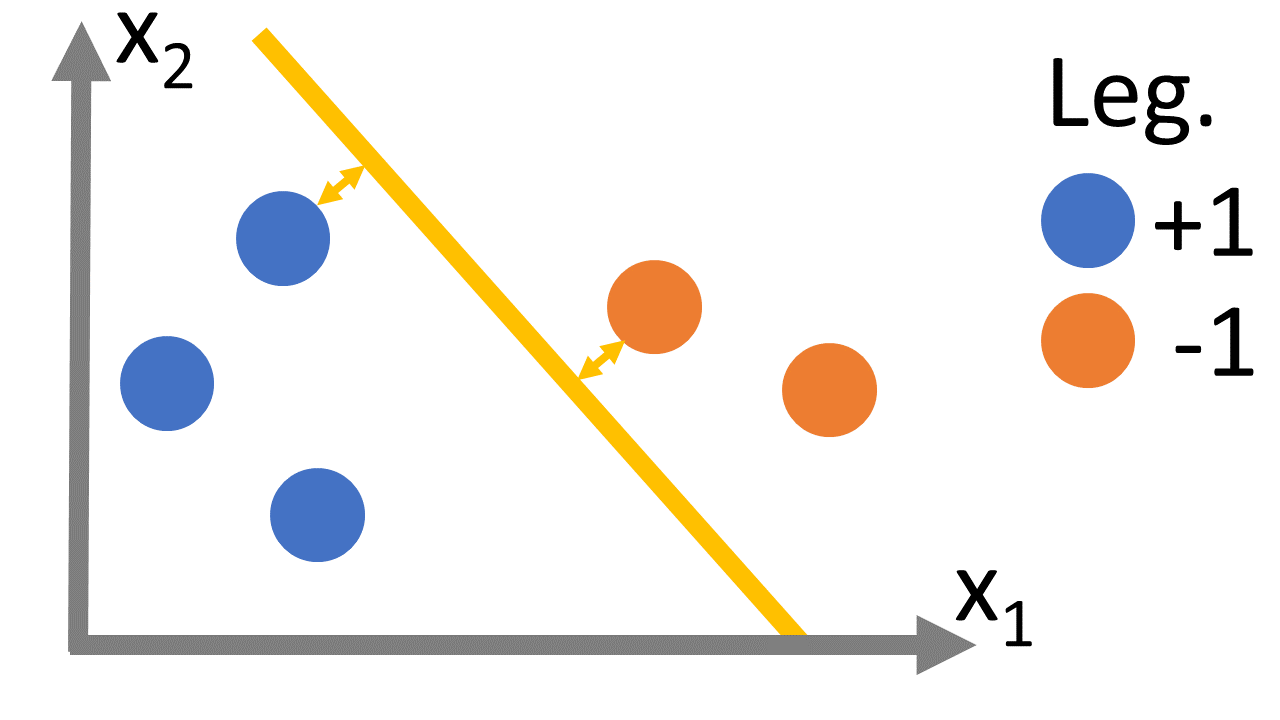
\includegraphics[width=0.5\textwidth]{PowerPoint/Folie3.png}
                % \caption{Beispiel eines Training-Sets}
                \label{definitionen:fig_2}
            }
        \end{figure}
    }\only<3>{
        \begin{figure}[h]
            \centering{
                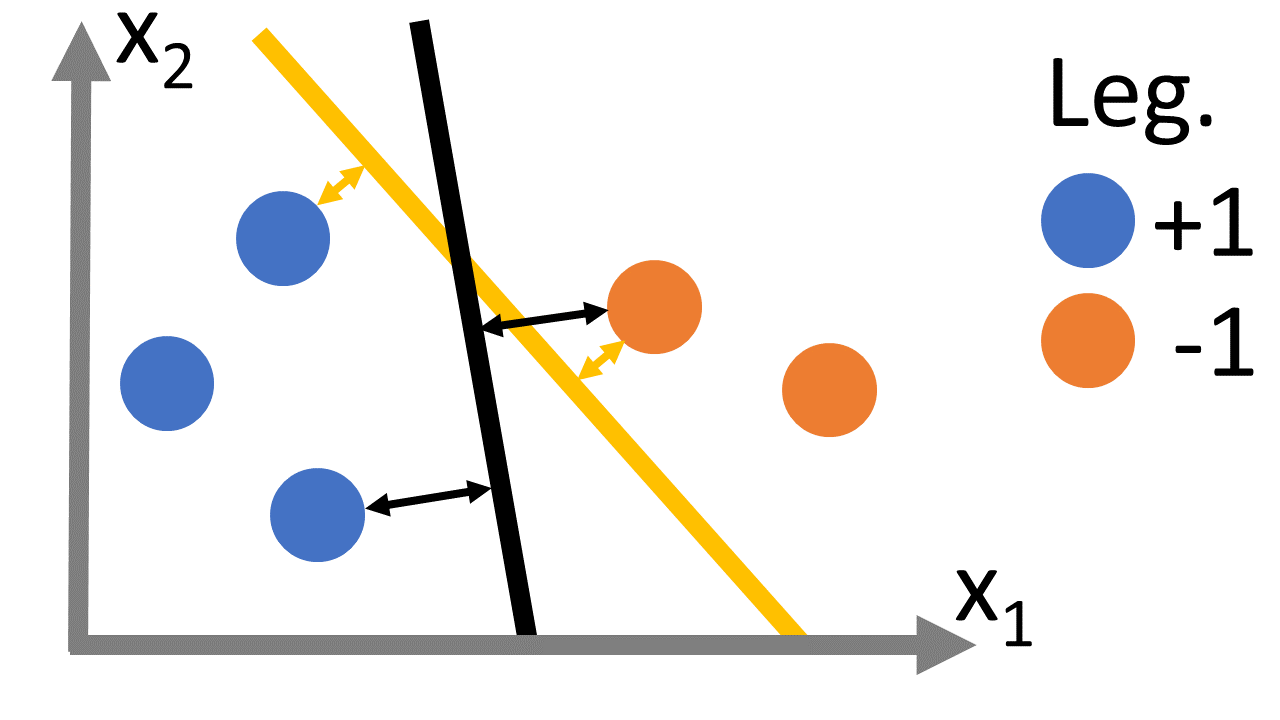
\includegraphics[width=0.5\textwidth]{PowerPoint/Folie4.png}
                % \caption{Beispiel eines Training-Sets}
                \label{definitionen:fig_3}
            }
        \end{figure}
    }\only<4>{
        \begin{figure}[h]
            \centering{
                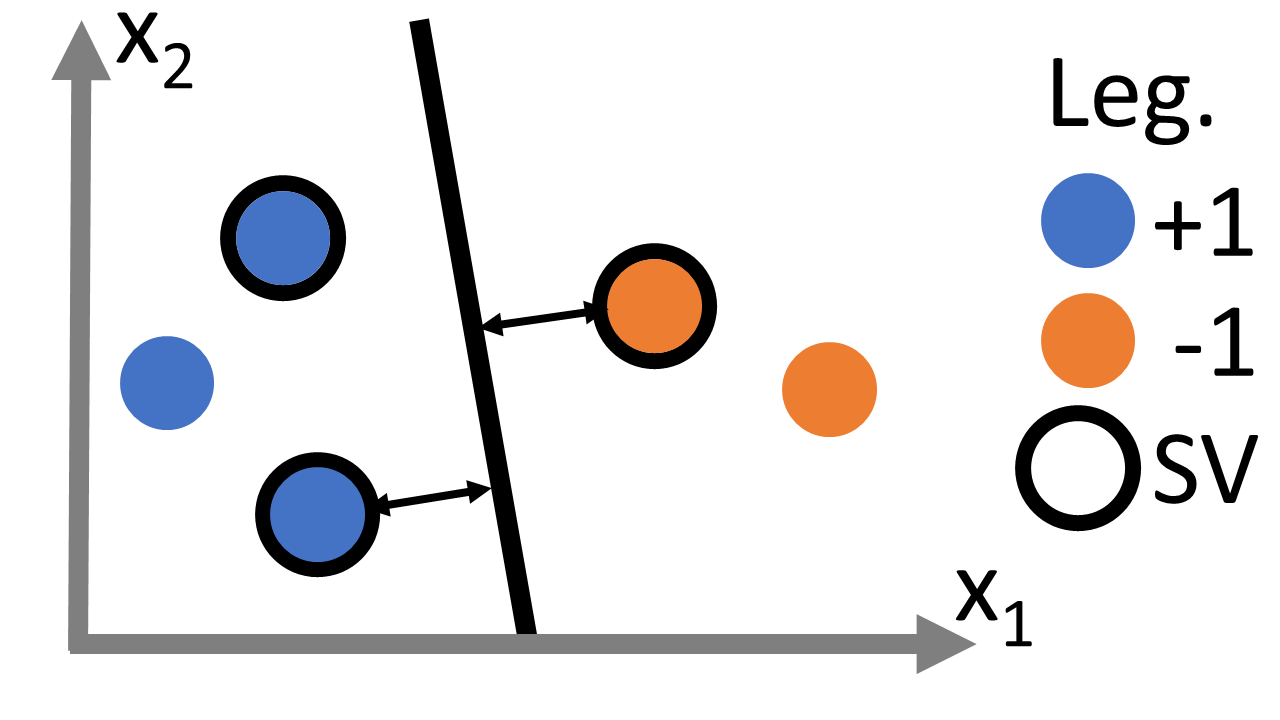
\includegraphics[width=0.5\textwidth]{PowerPoint/Folie5.png}
                % \caption{Beispiel eines Training-Sets}
                \label{definitionen:fig_4}
            }
        \end{figure}
    }

    \only<1>{
        \vspace{3mm}
        
        \begin{itemize}
            \item Wie trenne ich die beiden Klassen voneinander?
        \end{itemize}
    }

    % \only<2->{
    %     \vspace{3mm}

    %     \begin{itemize}
    %         \item Hyperebene: $ \boldsymbol{w} \cdot \boldsymbol{x} + b = 0 $
    %     \end{itemize}
    % }

    \only<2>{
        \vspace{2mm}

        \begin{itemize}
            \item Wie lege ich die Hyperebene am besten?
        \end{itemize}
    }

    \only<3-4>{
        \vspace{2mm}

        \begin{itemize}
            \item Anderer Name von Support Vector Machines: Large Margin Classifier
        \end{itemize}
    }
\end{frame}

%%%%%%%%%%%%%%%%%%%%%%%%%%%%%%%%%%%%%%%%%%%%%%%%%%%%%%%%%%%%%%%%%%%%%%%%%%%%%%%%
%Folie 4: Definitionen
%%%%%%%%%%%%%%%%%%%%%%%%%%%%%%%%%%%%%%%%%%%%%%%%%%%%%%%%%%%%%%%%%%%%%%%%%%%%%%%%
\begin{frame}
    \frametitle{Definitionen}

    \begin{figure}[h]
        \begin{minipage}{0.4\textwidth} 
            \begin{figure}[h]
                \centering{
                    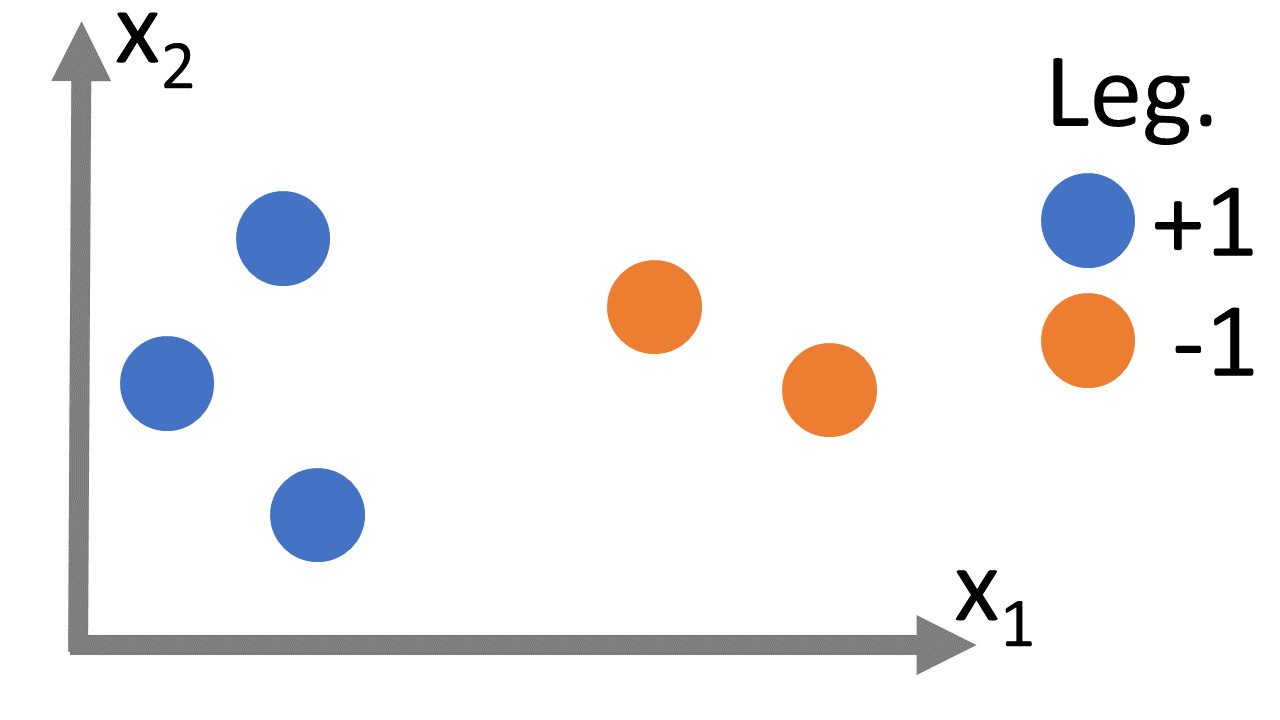
\includegraphics[width=\textwidth]{PowerPoint/Folie2.png}
                    % \caption{Beispiel eines Training-Sets}
                    \label{definitionen:fig_1}
                }
            \end{figure}
        \end{minipage}
        \hfill
        \begin{minipage}{0.4\textwidth}
            \begin{itemize}
                \item<2-> $m = 5$
                \item<2-> Trainingsset:
                    \begin{align*}
                        S &\in (\boldsymbol{x} \times \boldsymbol{y})^m \\
                        &=  \left( \begin{matrix}
                            1 & 0.5 & +1 \\
                            3.5 & 1 & -1 \\
                            & \vdots & \\
                        \end{matrix} \right) \\
                    \end{align*}
            \end{itemize} 
        \end{minipage}
    \end{figure}
    
    \begin{itemize}
        \item Anzahl an Trainingspunkten $ m \in \mathbb{R} $
        \item Input $ \boldsymbol{x} \in \mathbb{R}^N $
        \item Output $ \boldsymbol{y} \in \{ -1, +1 \} $
        \item Trainingsset $S \in (\mathbb{R}^N \times \{ -1, +1 \})^m $
        \item Trainingsset $S \in (\boldsymbol{x} \times \boldsymbol{y})^m $
    \end{itemize}

    \vspace{2mm}

    \begin{itemize}
        \item Hypothese
            \begin{align*}
                h: \boldsymbol{x} &\to \boldsymbol{y} \\
                \boldsymbol{x}_i &\mapsto \{ +1, -1 \} \\
            \end{align*}
    \end{itemize}
\end{frame}

%%%%%%%%%%%%%%%%%%%%%%%%%%%%%%%%%%%%%%%%%%%%%%%%%%%%%%%%%%%%%%%%%%%%%%%%%%%%%%%%
%Folie 5: Large Margin Classifier
%%%%%%%%%%%%%%%%%%%%%%%%%%%%%%%%%%%%%%%%%%%%%%%%%%%%%%%%%%%%%%%%%%%%%%%%%%%%%%%%
\begin{frame}
    \frametitle{Large Margin Classifier}

    \begin{figure}[h]
        \centering{
            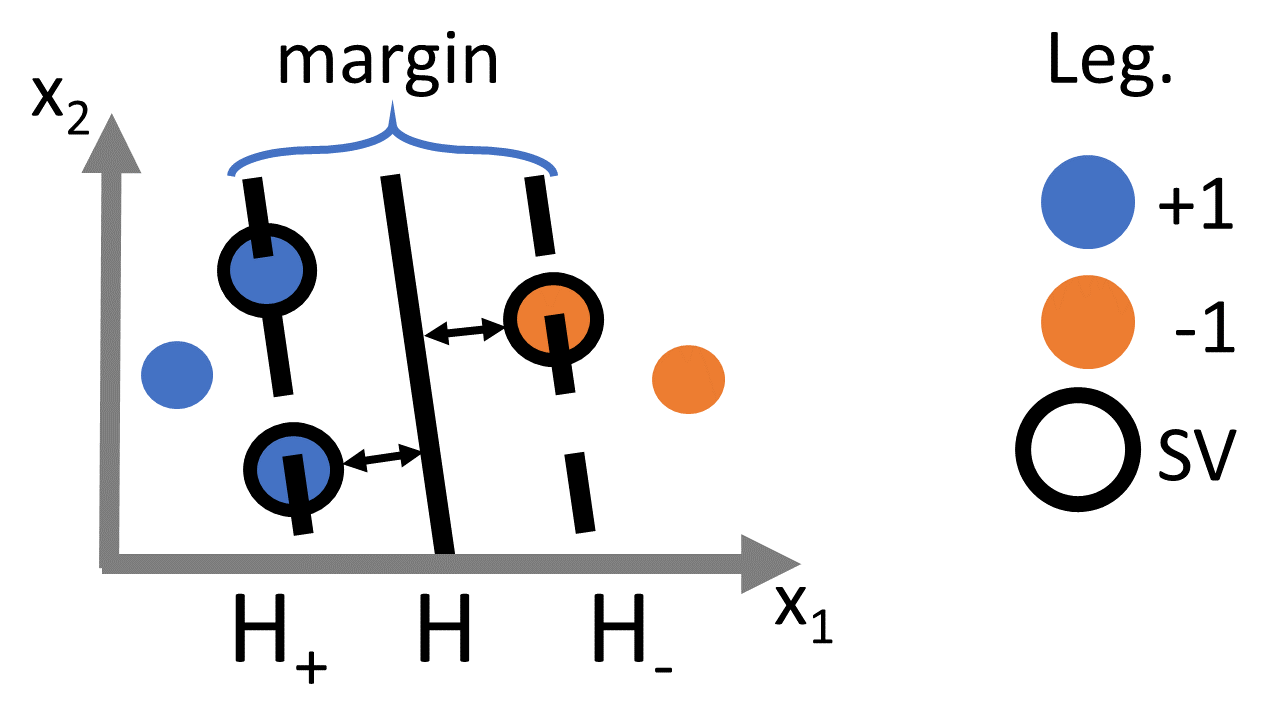
\includegraphics[width=0.5\textwidth]{PowerPoint/Folie7.png}
            % \caption{Beispiel eines Training-Sets}
            \label{large_marg_class:fig_1}
        }
    \end{figure}

    \vspace{3mm}

    \only<1> {
        \begin{itemize}
            \item Hyperebene: $ H' = \boldsymbol{w}' \cdot \boldsymbol{x} + b' = 0 $
            \item Gutter: $H_+$ und $H_-$
            \item Hyperbene frei skalierbar
        \end{itemize}
    }\only<2> {
        \begin{itemize}
            \item Hyperebene: $ H' = \boldsymbol{w}' \cdot \boldsymbol{x} + b' = 0 $
            \item Gutter constraint (GC):
                \begin{align*}
                    & \boldsymbol{w} \cdot \boldsymbol{x}_i + b = y_i, \quad \forall \text{ support vectors } \in \boldsymbol{x} \\
                    & y_i ( \boldsymbol{w} \cdot \boldsymbol{x}_i + b ) = 1 \quad \forall \text{ support vectors } \in \boldsymbol{x} \\
                \end{align*}
            \item Um GC zu erfüllen: $ \boldsymbol{w} $ und $b$ werden um $ c \in \mathbb{R} $ skaliert:
                \begin{align*}
                    & H = c ( \boldsymbol{w} \cdot \boldsymbol{x} + b ) = 0 \\
                    & \boldsymbol{w} = c \cdot \boldsymbol{w}' \\
                    & b = c \cdot b' \\
                \end{align*}
            \item $H$ heißt auch kanonische Hyperebene
        \end{itemize}
    }\only<3> {
        \begin{itemize}
            \item Kanonische Hyperebene: $ H = \boldsymbol{w} \cdot \boldsymbol{x} + b = 0 $
            \item Kanonische Hyperebene ermöglicht Klassifizierung:
                \begin{equation*}
                    h(x_i) = \begin{cases}
                        +1 & \text{ wenn } \boldsymbol{w} \cdot \boldsymbol{x}_i + b \geq 0 \\
                        -1 & \text{ wenn } \boldsymbol{w} \cdot \boldsymbol{x}_i + b \leq 0 \\
                    \end{cases}
                \end{equation*}
        \end{itemize}
    }
\end{frame}

%%%%%%%%%%%%%%%%%%%%%%%%%%%%%%%%%%%%%%%%%%%%%%%%%%%%%%%%%%%%%%%%%%%%%%%%%%%%%%%%
% Folie 6: Beispiel I
%%%%%%%%%%%%%%%%%%%%%%%%%%%%%%%%%%%%%%%%%%%%%%%%%%%%%%%%%%%%%%%%%%%%%%%%%%%%%%%%
\begin{frame}
    \frametitle{Beispiel I}

    \begin{figure}[h]
        \begin{minipage}{0.4\textwidth} 
            \only<1>{
                \begin{figure}[h]
                    \centering{
                        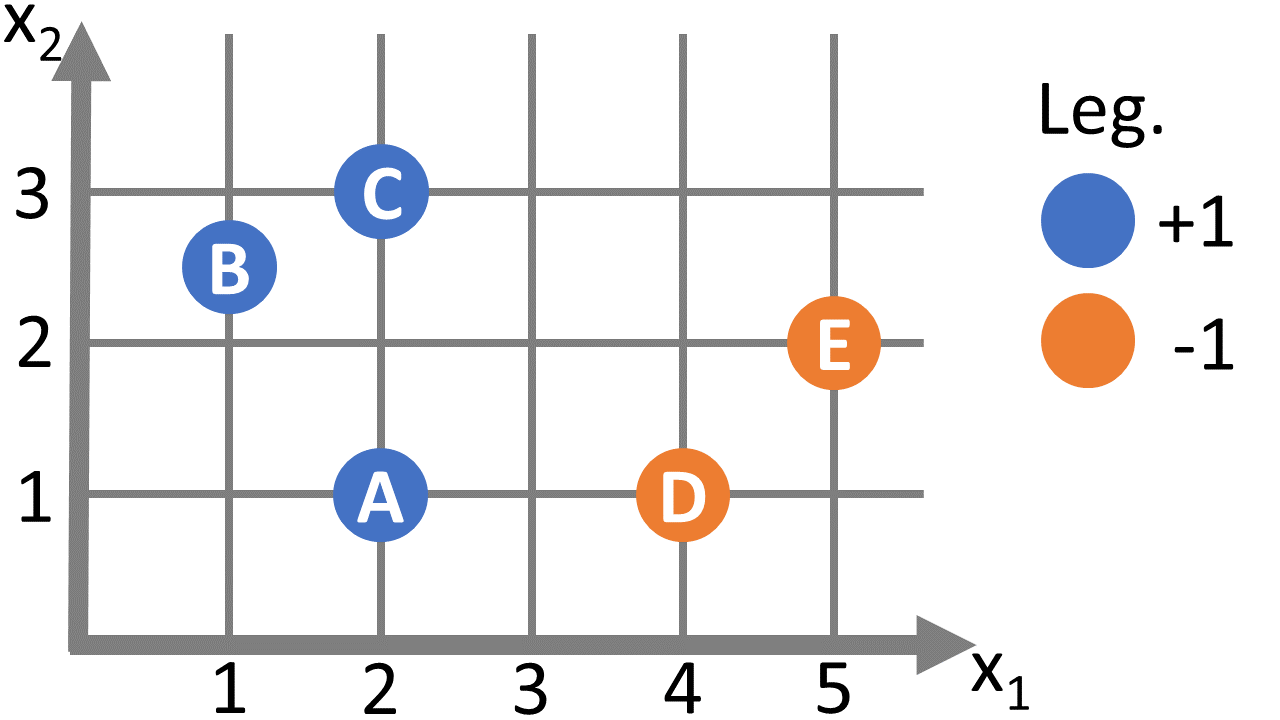
\includegraphics[width=\textwidth]{PowerPoint/Folie9.png}
                        % \caption{Beispiel eines Training-Sets}
                        \label{Bsp_1:fig_1}
                    }
                \end{figure}
            }\only<2->{
                \begin{figure}[h]
                    \centering{
                        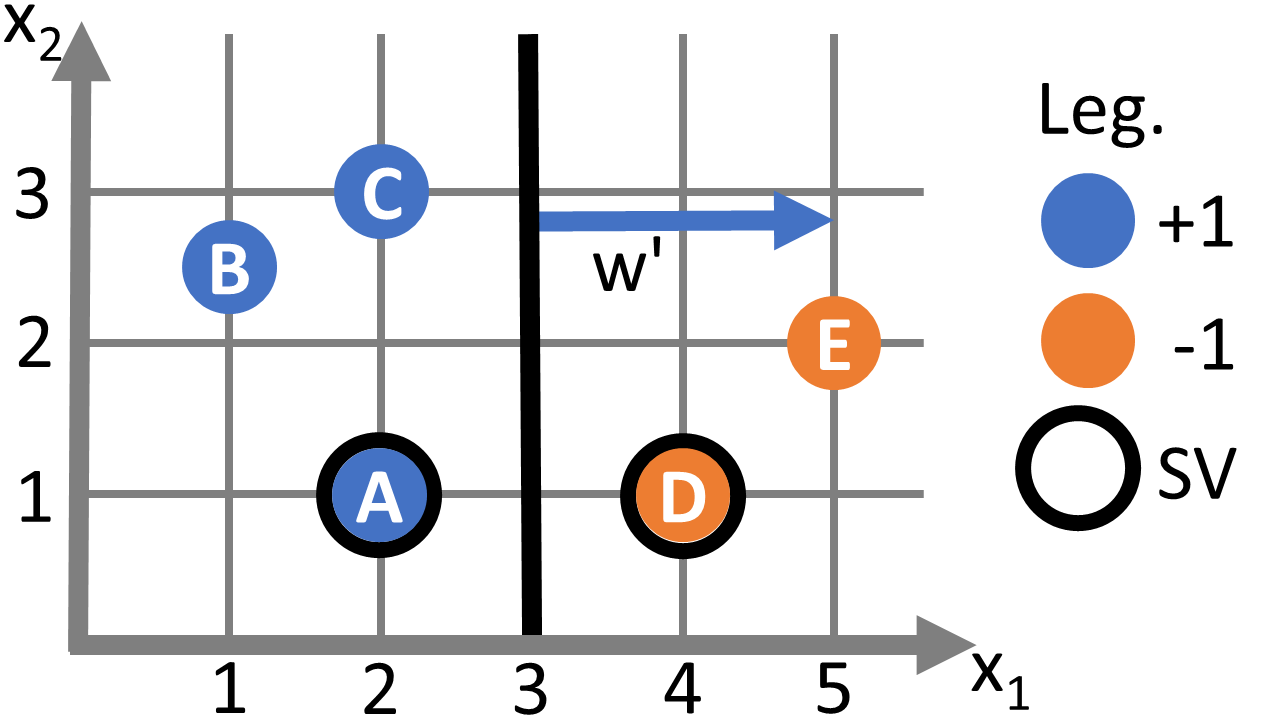
\includegraphics[width=\textwidth]{PowerPoint/Folie10.png}
                        % \caption{Beispiel eines Training-Sets}
                        \label{Bsp_1:fig_2}
                    }
                \end{figure}
            }
        \end{minipage}
        \hfill
        \begin{minipage}{0.4\textwidth}
            \begin{itemize}
                \item<1-> Hyperebene: $ H = \boldsymbol{w} \cdot \boldsymbol{x} + b = 0 $
                \item<1-> Gutter constraint: $ \boldsymbol{w} \cdot \boldsymbol{x}_i + b = y_i, \quad \forall \text{ s. v. } \in \boldsymbol{x} $
            \end{itemize} 
        \end{minipage}
    \end{figure}

    \begin{itemize}
        \item <2-> Graphische Bestimmung der Hyperebenenparameter:
            \begin{align*}
                x &= 3 \\
                \boldsymbol{w} &= \left( \begin{matrix}
                    2 \\
                    0 \\
                \end{matrix} \right) \\
                \left( \begin{matrix}
                    2 & 0 \\
                \end{matrix} \right) \cdot \left( \begin{matrix}
                    3 \\
                    0 \\
                \end{matrix} \right) + b = 0 &\Rightarrow b = -6 \\
            \end{align*}
    \end{itemize}
\end{frame}

%%%%%%%%%%%%%%%%%%%%%%%%%%%%%%%%%%%%%%%%%%%%%%%%%%%%%%%%%%%%%%%%%%%%%%%%%%%%%%%%
% Folie 7: Beispiel II
%%%%%%%%%%%%%%%%%%%%%%%%%%%%%%%%%%%%%%%%%%%%%%%%%%%%%%%%%%%%%%%%%%%%%%%%%%%%%%%%
\begin{frame}
    \frametitle{Beispiel II}

    \begin{figure}[h]
        \begin{minipage}{0.4\textwidth} 
            \only<1>{
                \begin{figure}[h]
                    \centering{
                        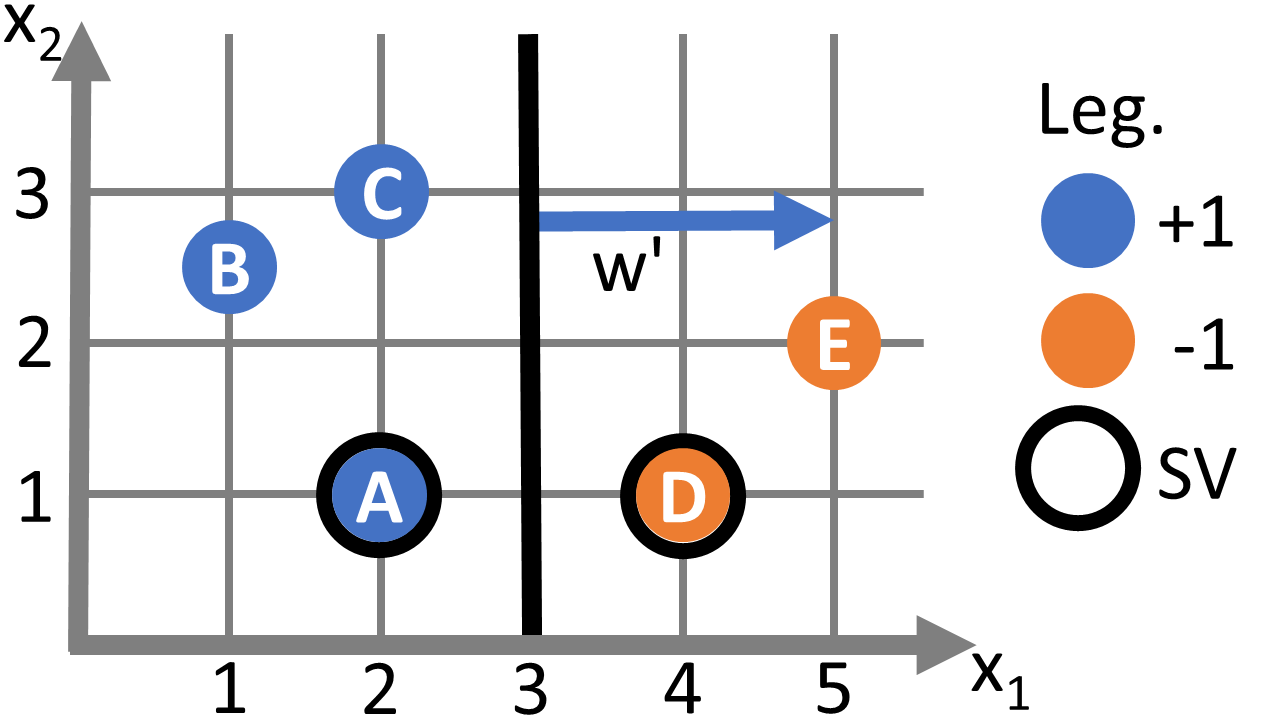
\includegraphics[width=\textwidth]{PowerPoint/Folie10.png}
                        % \caption{Beispiel eines Training-Sets}
                        \label{Bsp_1:fig_2}
                    }
                \end{figure}
            }\only<2->{
                \begin{figure}[h]
                    \centering{
                        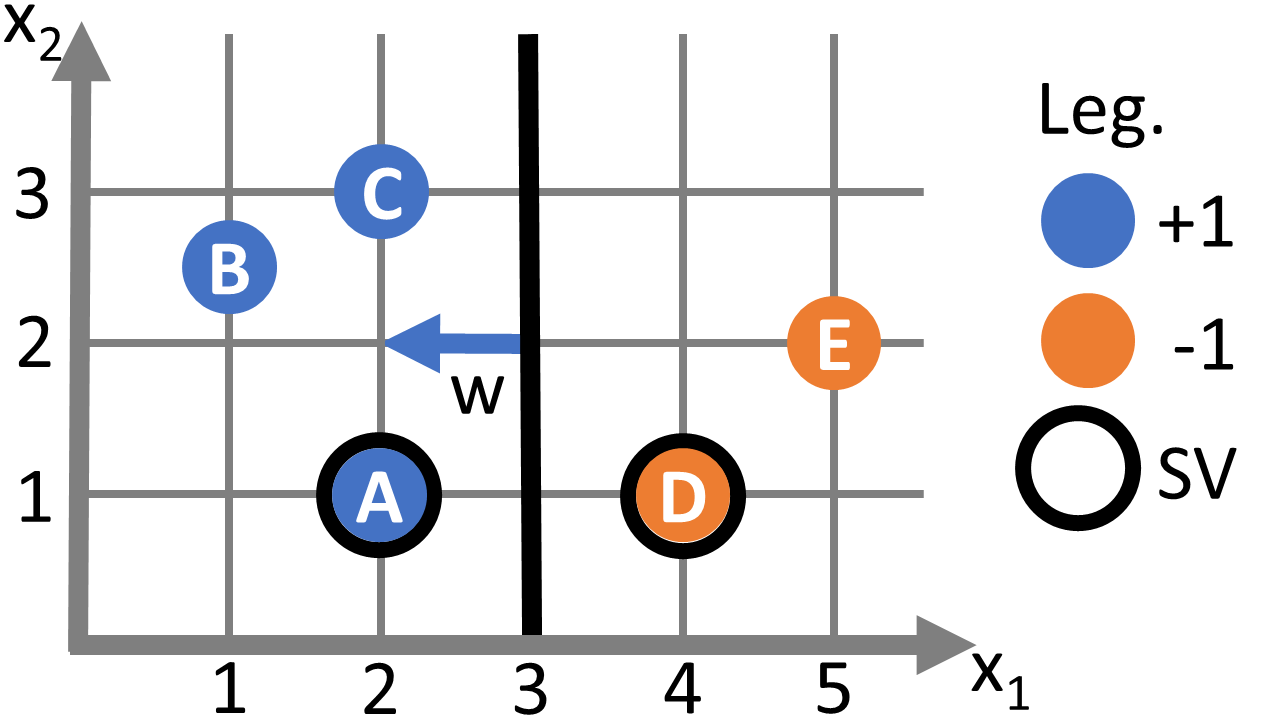
\includegraphics[width=\textwidth]{PowerPoint/Folie11.png}
                        % \caption{Beispiel eines Training-Sets}
                        \label{Bsp_1:fig_2}
                    }
                \end{figure}
            }
        \end{minipage}
        \hfill
        \begin{minipage}{0.4\textwidth}
            \begin{itemize}
                \item<1-> Hyperebene: $ H = \boldsymbol{w} \cdot \boldsymbol{x} + b = 0 $
                \item<1-> Gutter constraint: $ \boldsymbol{w} \cdot \boldsymbol{x}_i + b = y_i, \quad \forall \text{ s. v. } \in \boldsymbol{x} $
            \end{itemize} 
        \end{minipage}
    \end{figure}

    \begin{itemize}
        \item<1-> Berücksichtigen der Gutter constraint am Bsp. von Punkt $A$:
            \begin{align*}
                c \left( \left( \begin{matrix}
                    2 & 0 \\
                \end{matrix} \right) \cdot \left( \begin{matrix}
                    2 \\
                    1 \\
                \end{matrix} \right) - 6 \overset{!}{=} +1 \right) &\Rightarrow c = -0.5 \\
            \end{align*}
        \item<2-> Somit gilt für die kanonische Hyperebene:
            \begin{align*}
                \boldsymbol{w} &= \left( \begin{matrix}
                    -1 \\
                    0 \\
                \end{matrix} \right) \\
                b &= 3 \\ 
            \end{align*}
        \item<3-> Kontrolle mit Punkt $D$:
            \begin{align*}
                \left( \begin{matrix}
                    -1 & 0 \\
                \end{matrix} \right) \cdot \left( \begin{matrix}
                    4 \\
                    1 \\
                \end{matrix} \right) + 3 = -1
            \end{align*}
    \end{itemize}
\end{frame}

%%%%%%%%%%%%%%%%%%%%%%%%%%%%%%%%%%%%%%%%%%%%%%%%%%%%%%%%%%%%%%%%%%%%%%%%%%%%%%%%
% Folie 8: Beispiel III
%%%%%%%%%%%%%%%%%%%%%%%%%%%%%%%%%%%%%%%%%%%%%%%%%%%%%%%%%%%%%%%%%%%%%%%%%%%%%%%%
\begin{frame}
    \frametitle{Beispiel III}

    \begin{figure}[h]
        \begin{minipage}{0.4\textwidth} 
            \only<1->{
                \begin{figure}[h]
                    \centering{
                        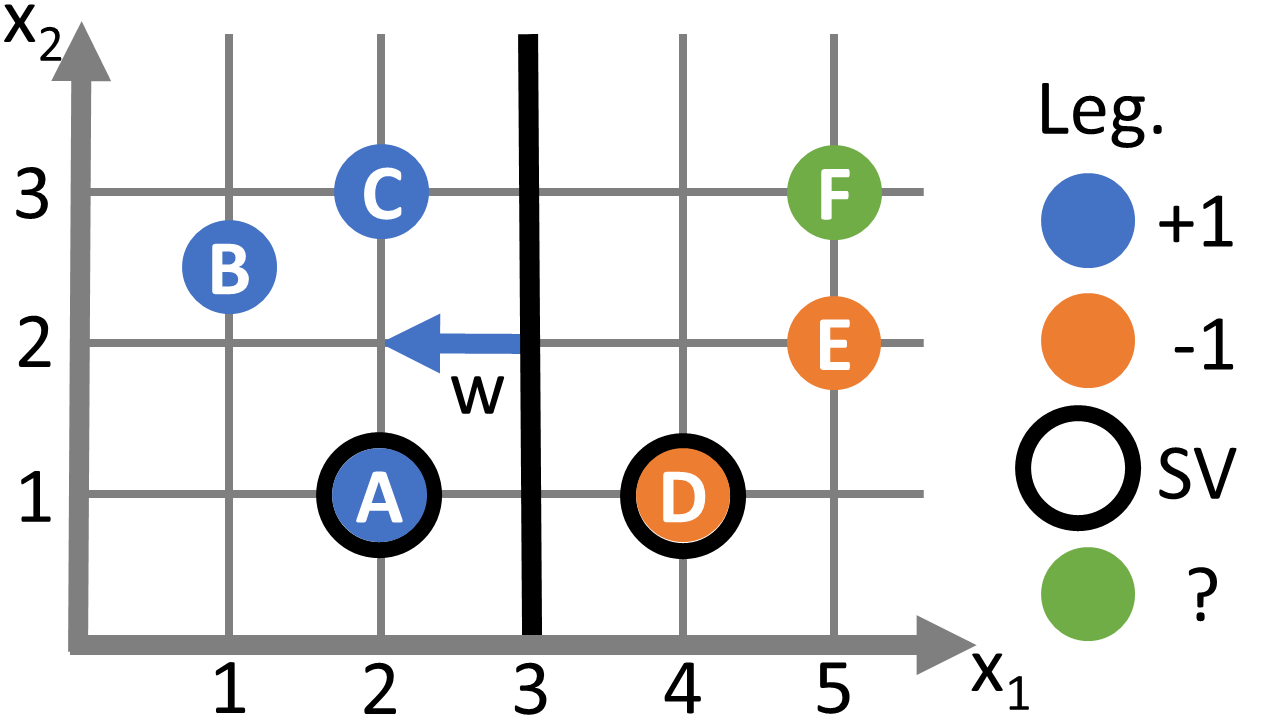
\includegraphics[width=\textwidth]{PowerPoint/Folie12.png}
                        % \caption{Beispiel eines Training-Sets}
                        \label{Bsp_1:fig_2}
                    }
                \end{figure}
            }
        \end{minipage}
        \hfill
        \begin{minipage}{0.4\textwidth}
            \begin{itemize}
                \item<1-> Klassifizierung:
                    \begin{equation*}
                        h(x_i) = \begin{cases}
                            +1 & \text{if } \boldsymbol{w} \cdot \boldsymbol{x}_i + b \geq 0 \\
                            -1 & \text{if } \boldsymbol{w} \cdot \boldsymbol{x}_i + b \leq 0 \\
                        \end{cases}
                    \end{equation*}
                \item<1-> Parameter der kanonischen Hyperebene
                    \begin{align*}
                        \boldsymbol{w} &= \left( \begin{matrix}
                            -1 \\
                            0 \\
                        \end{matrix} \right) \\
                        b &= 3 \\ 
                    \end{align*}
            \end{itemize} 
        \end{minipage}
    \end{figure}

    \begin{itemize}
        \item<1-> Klassifizierung von Punkt $F$:
            \begin{align*}
                \left( \begin{matrix}
                    -1 & 0 \\
                \end{matrix} \right) \cdot \left( \begin{matrix}
                    5 \\
                    3 \\
                \end{matrix} \right) + 3 = -2
            \end{align*}
        \item<1-> Punkt F gehört also zur Klasse $-1$.
    \end{itemize}
\end{frame}

%%%%%%%%%%%%%%%%%%%%%%%%%%%%%%%%%%%%%%%%%%%%%%%%%%%%%%%%%%%%%%%%%%%%%%%%%%%%%%%%
% Folie 9: Minimierungsproblem
%%%%%%%%%%%%%%%%%%%%%%%%%%%%%%%%%%%%%%%%%%%%%%%%%%%%%%%%%%%%%%%%%%%%%%%%%%%%%%%%
\begin{frame}
    \frametitle{Minimierungsproblem}

    \begin{figure}[h]
        \begin{minipage}{0.4\textwidth} 
            \only<1->{
                \begin{figure}[h]
                    \centering{
                        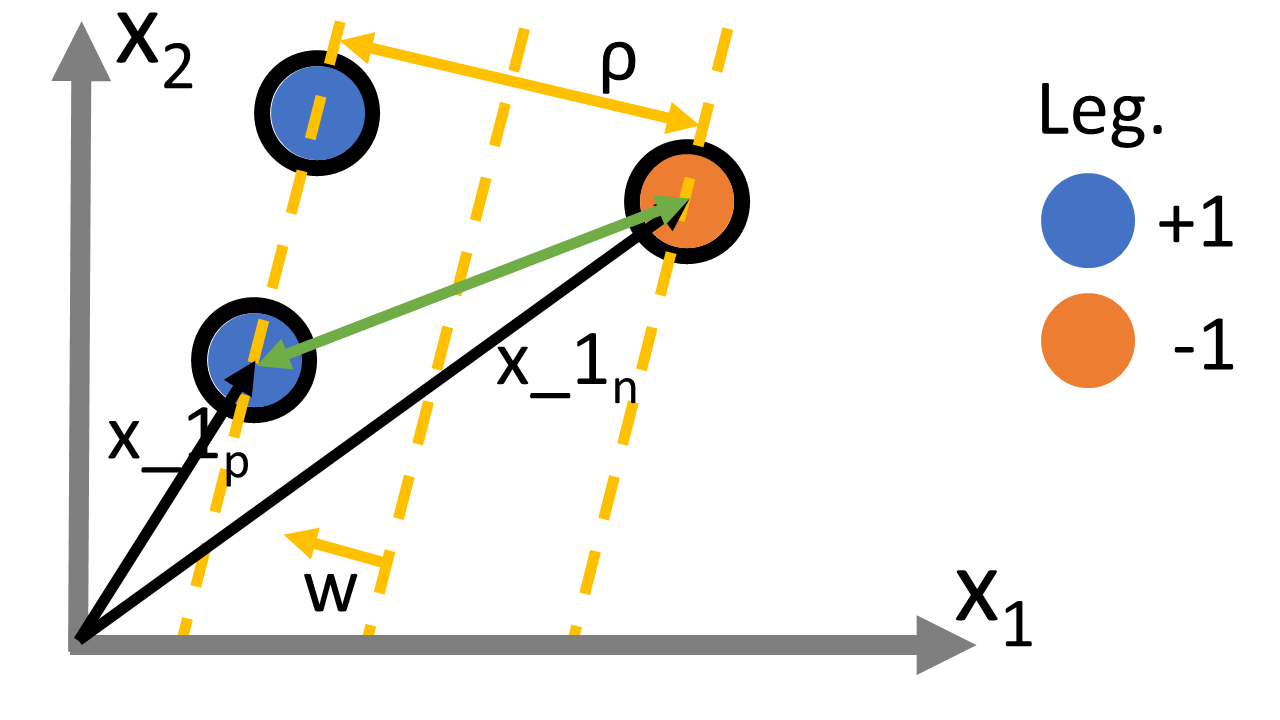
\includegraphics[width=\textwidth]{PowerPoint/Folie8.png}
                        % \caption{Beispiel eines Training-Sets}
                        \label{Min_Prob:fig_1}
                    }
                \end{figure}
            }
        \end{minipage}
        \hfill
        \begin{minipage}{0.4\textwidth}
            \begin{itemize}
                \item Projektionseigenschaft des Skalarprodukts
                \item Breite des margin $\rho$:
                    \begin{equation*}
                        \rho = (\boldsymbol{x_p} - \boldsymbol{x_n}) \cdot \frac{\boldsymbol{w}}{\Vert \boldsymbol{w} \Vert}
                    \end{equation*}
                \item Gutter constraint: 
                    \begin{equation*}
                        y_i ( \boldsymbol{w} \cdot \boldsymbol{x}_i + b ) = 1 \quad \forall \text{ support vectors } \in \boldsymbol{x}
                    \end{equation*}
            \end{itemize} 
        \end{minipage}

        \begin{itemize}
            \item $ \rho = \frac{2}{\Vert \boldsymbol{w} \Vert} $
            \item Ziel einer SVM: Maximiere den margin
                \begin{align*}
                    & \max \frac{2}{\Vert \boldsymbol{w} \Vert} \Leftrightarrow \min \Vert \boldsymbol{w} \Vert \Leftrightarrow \min \frac{1}{2} \Vert \boldsymbol{w} \Vert^2 \\
                    & \text{u.d.N. } y_i ( \boldsymbol{w} \cdot \boldsymbol{x}_i + b ) - 1 \geq 0 \\
                \end{align*}
        \end{itemize}
    \end{figure}
\end{frame}

%%%%%%%%%%%%%%%%%%%%%%%%%%%%%%%%%%%%%%%%%%%%%%%%%%%%%%%%%%%%%%%%%%%%%%%%%%%%%%%%
% Folie 10: Lagrange multipliers
%%%%%%%%%%%%%%%%%%%%%%%%%%%%%%%%%%%%%%%%%%%%%%%%%%%%%%%%%%%%%%%%%%%%%%%%%%%%%%%%
\begin{frame}
    \frametitle{Lagrange multipliers}

    \begin{itemize}
        \item Langrange multipliers:
            \begin{align*}
                L = \frac{1}{2} \Vert \boldsymbol{w} \Vert^2 - \sum \alpha_i \left[ y_i ( \boldsymbol{w} \cdot \boldsymbol{x}_i + b) - 1 \right] \\
            \end{align*}
        \item Suche nach den Extremum
            \begin{align*}
                \frac{\partial L}{\partial \boldsymbol{w}} = \boldsymbol{w} - \sum \alpha_i y_i \boldsymbol{x}_i = 0 &\Rightarrow \boldsymbol{w} = \sum_i \alpha_i y_i \boldsymbol{x}_i \\
                \frac{\partial L}{\partial b} = -\sum \alpha_i y_i = 0 &\Rightarrow \sum_i \alpha_i y_i = 0 \\
            \end{align*}
        \item $\boldsymbol{w}$ in $L$ eingesetzt:
            \begin{align*}
                L &= \frac{1}{2} (\sum_i \alpha_i y_i \boldsymbol{x}_i) \cdot (\sum_j \alpha_j y_j \boldsymbol{x}_j) - (\sum_i \alpha_i y_i \boldsymbol{x}_i) \cdot (\sum_j \alpha_j y_j \boldsymbol{x}_j) - \sum_i \alpha_i y_i b + \sum_i \alpha_i \\
                L &= \sum_i \alpha_i - \frac{1}{2} \sum_i \sum_j \alpha_i \alpha_j y_i y_j \boldsymbol{x}_i \cdot \boldsymbol{x}_j
            \end{align*}
        \item Ziel: $ \max L$
        \item Entscheidungsfunktion:
            \begin{align*}
                h(\boldsymbol{u}) = \sum_i \alpha_i y_i \boldsymbol{x}_i \cdot \boldsymbol{u} + b \begin{cases}
                    \geq 0 & \Rightarrow y_u = +1 \\
                    \leq 0 & \Rightarrow y_u = -1 \\
                \end{cases}
            \end{align*}
    \end{itemize}
\end{frame}

%%%%%%%%%%%%%%%%%%%%%%%%%%%%%%%%%%%%%%%%%%%%%%%%%%%%%%%%%%%%%%%%%%%%%%%%%%%%%%%%
% Folie 11: supportiveness values
%%%%%%%%%%%%%%%%%%%%%%%%%%%%%%%%%%%%%%%%%%%%%%%%%%%%%%%%%%%%%%%%%%%%%%%%%%%%%%%%
\begin{frame}
    \frametitle{Supportiveness values $\alpha$}

    \begin{itemize}
        \item Eigenschaften:
            \begin{align*}
                & \boldsymbol{\alpha} \geq 0 \\
                & \alpha_i \begin{cases}
                    > 0 & \text{ wenn } x_i \text{ ein support vector ist} \\
                    = 0 & \text{ sonst} \\
                \end{cases} \\
            \end{align*}
        \item $ \sum\limits_{\substack{ \text{s.v.} \\ i}} \alpha_i y_i  = 0 \Leftrightarrow \sum\limits_{\substack{ \text{pos. s.v.} \\ p}} \alpha_p  = \sum\limits_{\substack{ \text{neg. s.v.} \\ n}} \alpha_n $
        \item $ \sum\limits_i \alpha_i y_i \boldsymbol{x}_i = \boldsymbol{w} \Leftrightarrow \boldsymbol{w} = \sum\limits_p \alpha_p \boldsymbol{x}_p - \sum\limits_n \alpha_n \boldsymbol{x}_n $
    \end{itemize}

    \vspace{3mm}

    \only<2>{
        \begin{figure}[h]
            \begin{minipage}{0.4\textwidth} 
                \begin{figure}[h]
                    \centering{
                        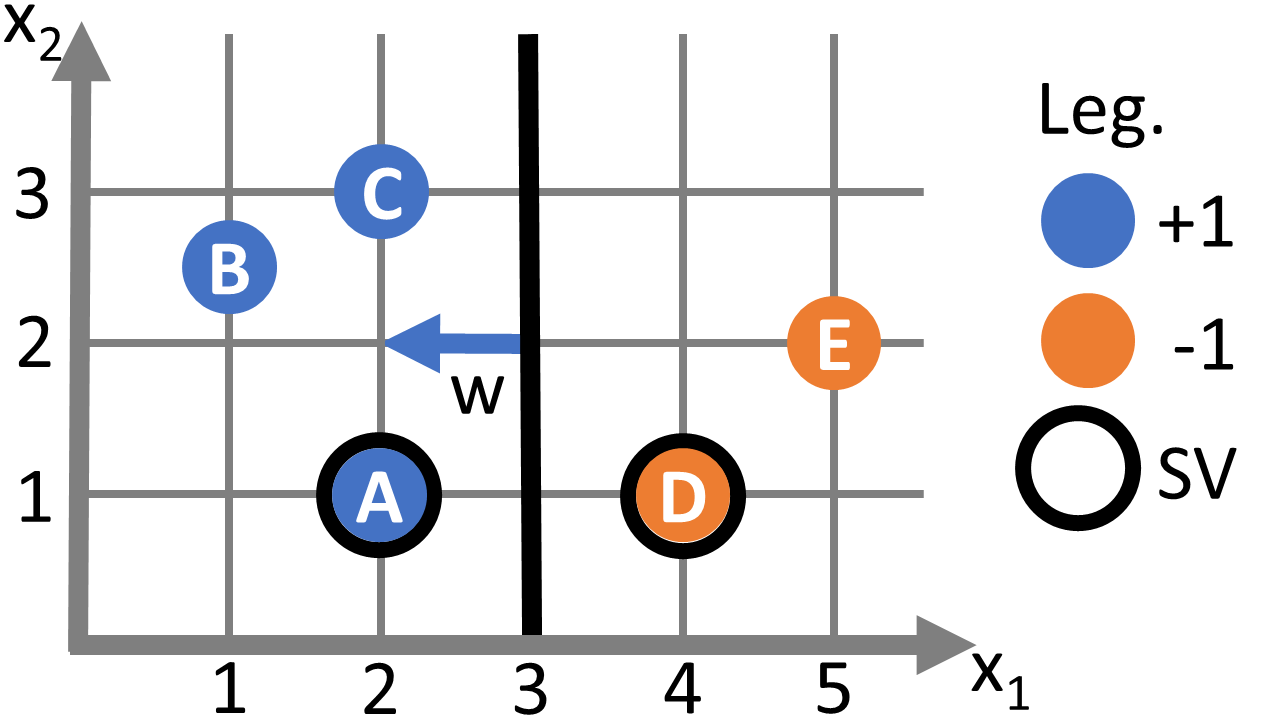
\includegraphics[width=\textwidth]{PowerPoint/Folie11.png}
                        % \caption{Beispiel eines Training-Sets}
                        \label{Bsp_1:fig_2}
                    }
                \end{figure}
            \end{minipage}
            \hfill
            \begin{minipage}{0.4\textwidth}
                \begin{itemize}
                    \item Berechnung von $\alpha_A$ und $\alpha_D$ ergibt:
                        \begin{align*}
                            \alpha_A &= 0.5 \\
                            \alpha_D &= 0.5
                        \end{align*}
                \end{itemize}

                \begin{itemize}
                    \item Berechnung von $\alpha_C$ ergibt:
                        \begin{align*}
                            \alpha_C = 0
                        \end{align*}
                \end{itemize}
            \end{minipage}
        \end{figure}
    }
\end{frame}

%%%%%%%%%%%%%%%%%%%%%%%%%%%%%%%%%%%%%%%%%%%%%%%%%%%%%%%%%%%%%%%%%%%%%%%%%%%%%%%%
% Folie 12: Zusammenfassung
%%%%%%%%%%%%%%%%%%%%%%%%%%%%%%%%%%%%%%%%%%%%%%%%%%%%%%%%%%%%%%%%%%%%%%%%%%%%%%%%
\begin{frame}
    \frametitle{Zusammenfassung}

    \begin{itemize}
        \item Kanonische Hyperebene:
            \begin{align*}
                \boldsymbol{w} \cdot \boldsymbol{x} + b = 0
            \end{align*}
        \item Gesucht: Parameter $\boldsymbol{w}$ und $b$
        \item Supportive values $\alpha$:
            \begin{align*}
                \boldsymbol{w} = \sum_i \alpha_i y_i \boldsymbol{x}_i \\
                \sum_i \alpha_i y_i = 0 \\
            \end{align*}
        \item Entscheidungsfunktion $H$:
            \begin{align*}
                h(\boldsymbol{u}) = \sum_j \alpha_j y_j \boldsymbol{x}_j \cdot \boldsymbol{u} + b \begin{cases}
                    \geq 0 & \Rightarrow y_u = +1 \\
                    \leq 0 & \Rightarrow y_u = -1 \\
                \end{cases}
            \end{align*}
        \item Supportvektoren
            \begin{align*}
                & y_i (\sum_j \alpha_j y_j \boldsymbol{x}_j \cdot \boldsymbol{x}_i + b) = 1 \quad \forall \text{ s.v. } \boldsymbol{x}_i \in \boldsymbol{x} \\
                & \alpha_i \begin{cases}
                    > 0 & \text{ wenn } x_i \text{ ein support vector ist} \\
                    = 0 & \text{ sonst} \\
                \end{cases} \\
            \end{align*}
    \end{itemize}
\end{frame}


\end{document}

